%% chapitre 1
\documentclass[a4paper,dvips]{article}
\usepackage{ucs}
\usepackage[utf8x]{inputenc}
\usepackage[T1]{fontenc}
\usepackage[dvips]{graphicx}
\usepackage{amsmath}
\usepackage{psfrag}
\usepackage{pst-all}
\begin{document}
\begin{figure*}[ht]
    \begin{flushleft}
        \psfrag{D}{$D$}
        \psfrag{dD}{$\partial D$}
        \psfrag{M}{$M$}
        \psfrag{n}{$\vec{n}$}
        \psfrag{T}{$\vec{T}$}
        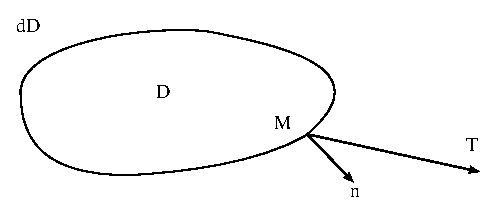
\includegraphics{T1_Ch01-0001.eps}
    \end{flushleft}
    \label{fig:T1_Ch01-0001}
\end{figure*}
\begin{figure*}[ht]
    \begin{flushleft}
        \psfrag{D1}{$D_I$}
        \psfrag{D2}{$D_{II}$}
        \psfrag{D3}{$D_{III}$}
        \psfrag{Vdt}{$\vec{V} \mathrm{d}t$}
        \psfrag{Dtdt}{$D\left( t+\mathrm{d}t \right)$}
        \psfrag{Dt}{$D\left( t \right)$}
        \psfrag{t}{\footnotesize $\theta$}
        \psfrag{n}{$\vec{n}$}
        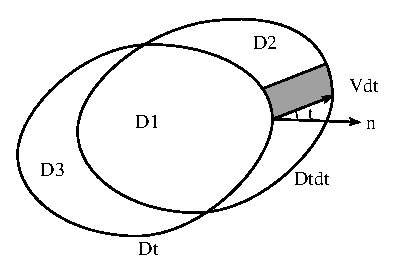
\includegraphics{T1_Ch01-0002.eps}
    \end{flushleft}
    \label{fig:T1_Ch01-0002}
\end{figure*}
\end{document}
